\section{Methoden}
	
	Dieser Abschnitt befasst sich mit dem Aufbau des Versuches und den dabei auftretenden Unsicherheiten.
	
	\subsection{Aufbau}	
		
		\begin{figure}[ht]
			\centering
			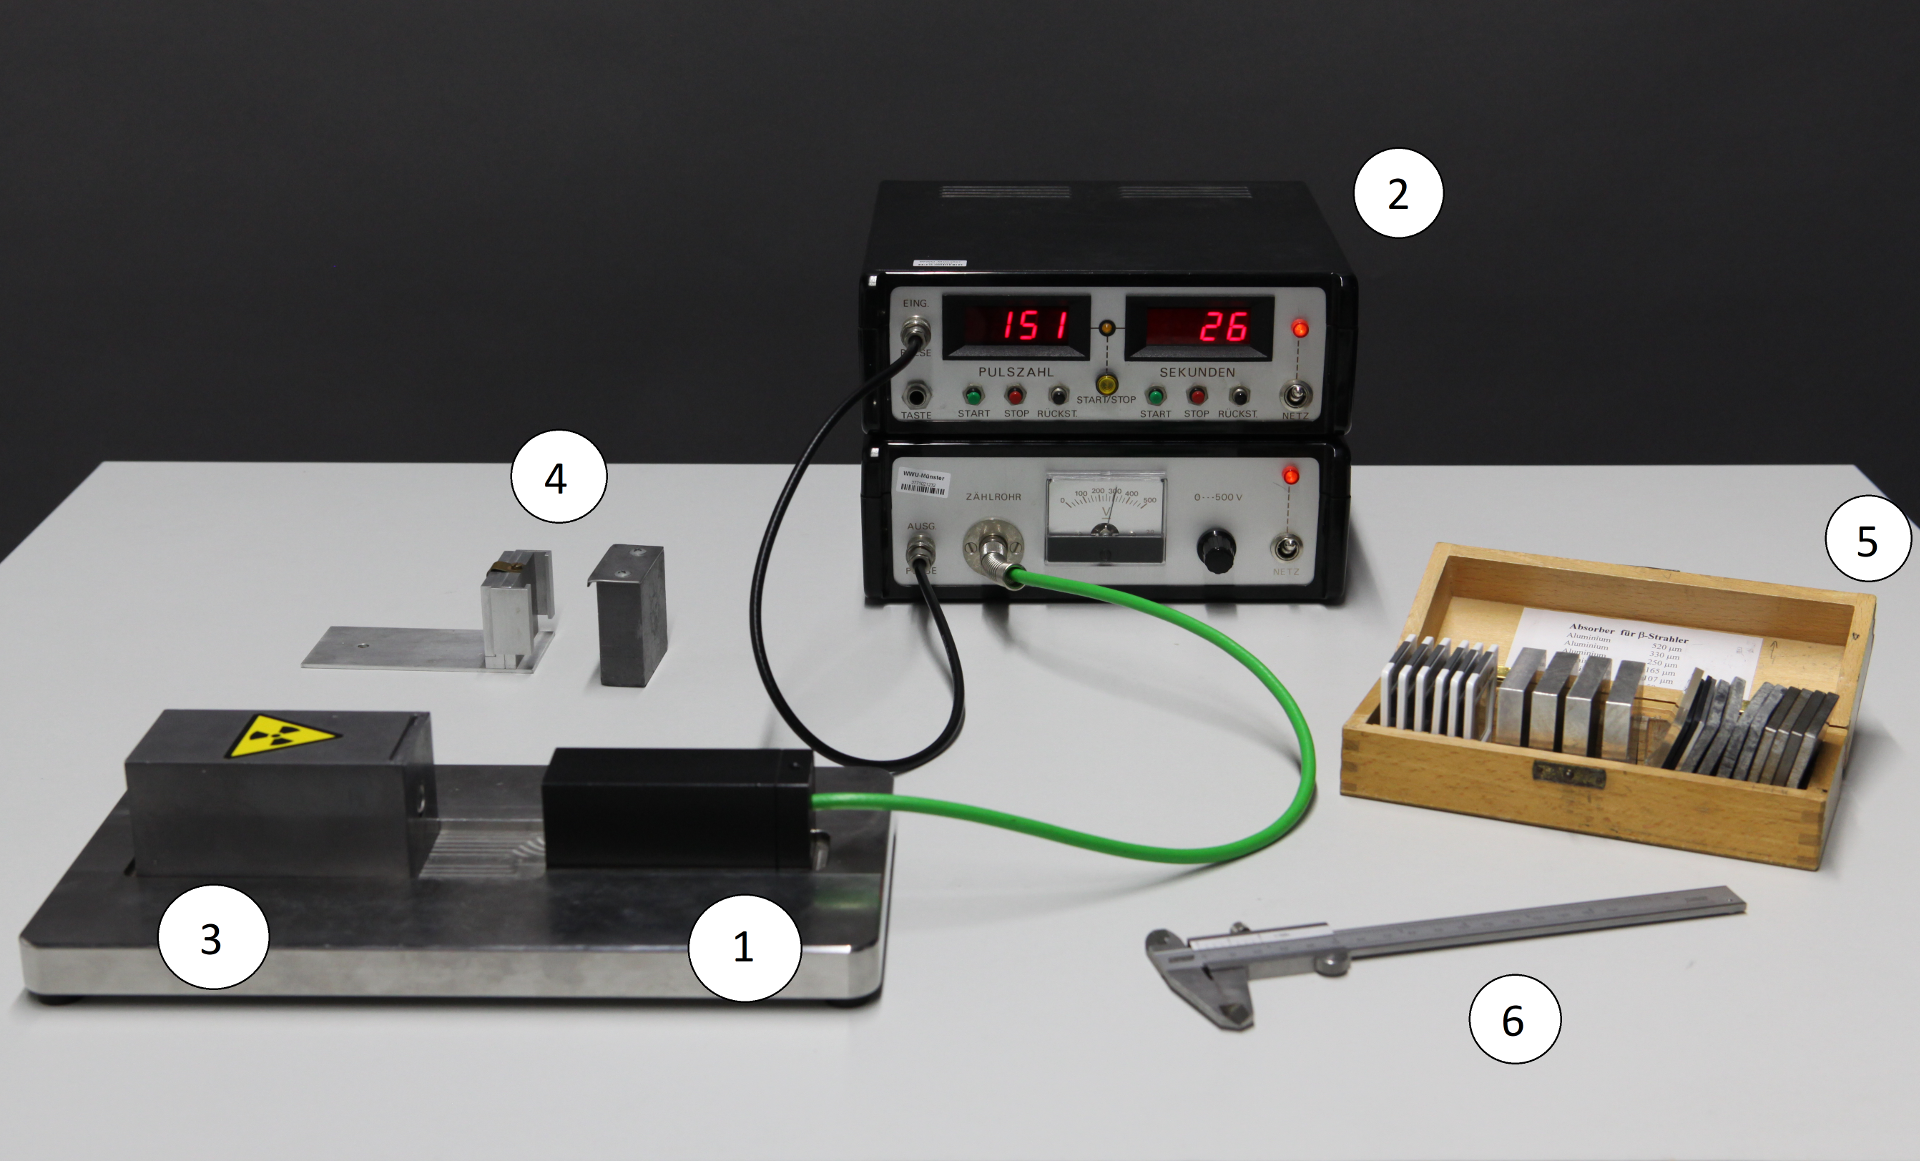
\includegraphics[width=\textwidth]{Aufbau.png}
			\caption{Aufbau des Versuches. \cite{WWU}}
			\label{fig:Aufbau}	
		\end{figure}
		Der Aufbau, wie er in in Abb. \ref{fig:Aufbau} dargestellt ist, besteht im Wesentlichen aus einem Geiger-Müller-Zählrohr (1) mit zugehöriger Messapparatur (2) und einem radioaktiven Präparat, welches in geringem Abstand (wenige Zentimeter) von dem Zählrohr steht.
		Bei den verwendeten radioaktiven Präparaten handelt es sich um den $\beta$-Strahler $^{90}$Sr (4) und den $\gamma$-Strahler $^{137}$Cs (3).
		Zwischen dem Zählrohr und das Präparat können kleine Platten aus Absorbermaterialien (5) platziert werden, sodass eine Messung der Impulsrate in Abhängigkeit der Dicke des Absorbers möglich ist.
		Zur Messung der Dicke der Platten steht eine Schiebelehre (6) zur Verfügung.
		
		Mit Hilfe der Messapparatur die an das Zählrohr geschlossen ist, lassen sich die Anzahl der Impulse bzw. radioaktiven Ereignissen wie auch die vergangene Zeit einfach von einem Digitaldisplay ablesen.
		Zudem lässt sich dort die Spannung an dem Zählrohr einstellen.
		
		Zur Messung der natürlichen Strahlung wird das Präparat, welches vor dem Zählrohr platziert ist, entfernt.
				
	\subsection{Unsicherheiten}
	
		Jegliche Unsicherheiten werden nach GUM bestimmt und berechnet\footnote{Die Gleichungen dazu finden sich im Anhang unter \ref{fig:GUM_combine}, \ref{fig:GUM_formula}.}.
		Für die Unsicherheitsrechnungen wurde die Python Bibliothek "uncertainties" herangezogen, welche den Richtlinien des GUM folgt.
	
		Für digitale Messungen wird eine Unsicherheit von $u(X) = \frac{\Delta X}{\sqrt{3}}$ angenommen, bei analogen eine von $u(X) = \frac{\Delta X}{\sqrt{6}}$.

\section{Durchführung und Datenanalyse}
		
	Die Zeit bzw. die Zahl der Ereignisse wurde bei allen Messungen so gewählt, dass die relative Unsicherheit unter 4\%, für alle Messwerte liegt.
	Das Wechseln oder Entfernen der radioaktiven Präparate wurde von dem Betreuer durchgeführt.
	
	Zur Bestimmung der Zählrohrcharakteristik wurde der $\beta$-Strahler $^{90}$Sr verwendet und für verschiedene Spannungen die Anzahl der Ereignisse nach \SI{94}{\second} aufgetragen. % TODO Unsicherheit
	Eine Darstellung der Messwerte ist der Abb. \ref{label} zu entnehmen. % TODO Label
	Diese Kennlinie zeigt, dass zur Messung der Radioaktivität mindestens eine Spannung von \SI{0}{\volt} anliegen muss, diese nennt sich Einsatzspannung. % TODO Wert
	Auch das charakteristische Plateau nach dem Erreichen dieser Spannung ist der Kurve zu entnehmen.
	Zudem ließen sich nur Werte bis zu \SI{500}{\volt} einstellen, da höhere Spannungen zur Beschädigung oder gar Zerstörung des Zählrohrs führen könnten. %TODO Unsicherheit
	
	Zur Messung der natürlichen Radioaktivität wurde das radioaktive Präparat entfernt und 200 mal die Anzahl der Ereignisse innerhalb von \SI{10}{\second} aufgenommen.
	Aus dieser Verteilung folgen der Mittelwert $ $ wie auch die empirische Standardabweichung $ $. %TODO Werte
	Diagramme der absoluten und relativen Häufigkeitsverteilung sind in Abb. \ref{label} vorzufinden. %TODO Label
	Zur Bestimmung der Werte wurde die Poisson-Verteilung herangezogen. % TODO wie
	Mit Hilfe der mittleren Untergrundaktivität, die aus der natürlichen Radioaktivität hervorgegangen ist, ließ sich nun eine Korrektur, für die folgenden Messungen durchführen.
	
	Zur Bestimmung des Absorptionskoeffizienten $\mu_\gamma$ von Blei wurde die Impulsrate $a_\gamma (x)$ des $\gamma$-Präparats $^{137}$Cs in Abhängigkeit der Schichtdicke des Blei-Absorbers aufgenommen.	
	Hierbei wurde die Zeit gemessen, die benötigt wurde um ca. 650 Ereignisse in dem Zählrohr auszulösen, um die Impulsrate mit einer relativen Unsicherheit unter 4\% aufzunehmen.
	Zusätzlich wurde die Spannung an dem Zählrohr so gewählt, dass sie mit $\SI{400}{\volt}$ ca. \SI{100}{\volt} über der Einsatzspannung, mitten auf dem Plateau der Zählrohrcharakteristik liegt.
	Nach jeder Messreihe wurde eine weitere Platte hinzugefügt und eine neue Reihe gestartet, sodass die Impulsrate in Abhängigkeit der Schichtdicke aufgetragen werden konnte.
	Dazu standen vier Blei-Platten zur Verfügung.
	Abb. \ref{label} stellt das Verhältnis logarithmisch aufgetragen dar. % TODO Label
	Da es sich bei steigender Schichtdicke um einen exponentiellen Abfall der Ereignisse handeln sollte, lässt sich der Absorptionskoeffizient aus der Steigung des Graphen bestimmen.
	Diese beläuft sich bei dem Blei auf $\mu_\gamma = $ % TODO Wert
	
	Analog verlief die Messung der Impulsraten $a_\beta (x)$ des $\beta$-Präparats $^{90}$Sr in Abhängigkeit der Schichtdicken von Aluminium, Plexiglas und Gummi.
	Für die letzteren beiden, wurde die Messung jedoch nur für je eine Schicht durchgeführt.
	Eine graphische Darstellung der Messung ist in Abb. \ref{label} vorzufinden. % TODO Label
	Die sich dadurch berechneten Absorptionskoeffizienten sind in Tab. \ref{tab:Werte} verzeichnet. % TODO Label
	
	\begin{table}
		\caption{In dieser Tabelle sind die ermittelten Absorptionskoeffizienten und die zugehörigen Literaturwerte\cite{temp} aufgetragen.}
		\label{tab:Werte}
		\centering
		\begin{tabular}{c|c|c|c|c}					
				& $\mu_\gamma$ Blei &  $\mu_\beta$ Aluminium & $\mu_\beta$ Plexiglas &$\mu_\beta$ Gummi \\
			\hline	
			ermittelt & \SI{0}{} & \SI{0}{} & \SI{0}{} & \SI{0}{} \\
			Literaturwert & \SI{0}{} & \SI{0}{} & \SI{0}{} & \SI{0}{} \\
			\hline
			Abweichung & 0\% & 0\% & 0\% & 0\% \\		
		\end{tabular}
	\end{table}
	
\section{Diskussion}
	
	Nun stellt sich die Frage, ob die Ergebnisse dem Ziel dieser Untersuchung genügen.
	
	Wird dazu zunächst die aufgenommene Zählrohrcharakteristik betrachtet, so lässt sich der zu erwartende Verlauf klar in dieser erkennen.
	Bis zur Einsatzspannung werden keine Impulses gemessen und die Werte, welche auf dem Plateau vorzufinden sind, liegen alle innerhalb ihrer Unsicherheiten.
	
	Die 
	
	% Aufnahme der natürlichen Strahlung
	% Gamma-Strahler, mit Blei
	% Beta-Strahler mit Aluminium, Plexiglas und Gummi , Blei als Absorber?
	